\documentclass[../../D1.tex]{subfiles}

\begin{document}
Initial software design/sketch of research Methodology

Functional / Non-functional requirements

High level framework design



Experimental data flow

benchmark framework

training and benchmark system

\subsection{Optimisation and Benchmarking suite}\label{sec:ERdiagram}
%This section will display a high level design on the benchmarking and optimisation suite.

Figure~\ref{fig:benchcycle} shows an entity relationship diagram to depict the benchmark and optimisation suite, either a hand crafted initial set of paramaters are provided to a \emph{Training Agent} or they could be randomly initialised at the start of the optimisation cycle.
This diagram also applies for the first set of experimental benchmarks (without an optimiser), in this case the \emph{Training Agent} will only train once with the specified compression parameters, and the cycle would terminate when the metrics are sent to Weights and Biases.

\begin{figure}[H]
    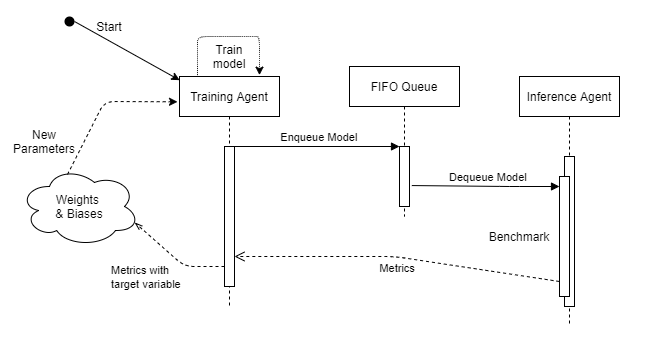
\includegraphics[width=1\textwidth]{dfd.png}
    \caption{Parameter optimisation ER diagram}
    \label{fig:benchcycle}
\end{figure}

Using this system we could theoretically benefit from adding new \emph{Training Agents} to the pool of agents until the consumers \emph{Inference Agent} are unable to clear the queue.
We intend to utilise at least two GPU, and one CPU \emph{Training Agents}, with a single \emph{Inference Agent}


\end{document}